%===============================================================
% chap2.tex — Phần cứng
%===============================================================
\pagestyle{fancy}
\chapter{CƠ SỞ PHẦN CỨNG}

\section{Sơ đồ khối chức năng}
Hệ thống gồm các khối sau:
\begin{enumerate}\itemsep0pt
	\item \textbf{Vòng bít và đường khí nối:} chứa áp suất làm xẹp động mạch và truyền áp tới cảm biến.
	\item \textbf{Cảm biến MPX5050:} chuyển áp suất tương đối thành điện áp tương tự (khảo sát đường đặc tuyến trong datasheet).
	\item \textbf{ADC ADS1115:} chuyển đổi điện áp với độ phân giải 16-bit; giao tiếp I\textsuperscript{2}C với MCU (địa chỉ thiết bị mặc định 0x48 khi chân ADDR nối GND).
	\item \textbf{Vi điều khiển STM32F103 (Blue Pill):} đọc ADS1115, điều khiển PWM bơm và van, đọc nút nhấn, điều khiển LED và truyền thông UART.
	\item \textbf{Nguồn và điều kiện tiếp đất:} đảm bảo MPX5050 và ADC có tham chiếu ổn định; layout PCB tuân thủ khuyến nghị của nhà sản xuất để giảm nhiễu đo lường.
\end{enumerate}

\section{Giao tiếp và chân cắm chính}
Theo cấu hình mặc định trong firmware (\texttt{board\_config.h}):
\begin{itemize}\itemsep0pt
	\item UART1 115200~bps: PA9 (TX), PA10 (RX).
	\item I2C1: PB6 (SCL), PB7 (SDA) nối ADS1115.
	\item Timer 3 PWM: PA6 kênh bơm, PA7 kênh van (điều chỉnh duty để servo tốc độ bơm/xả).
	\item Nút tác động mức thấp (kéo lên nội bộ): PA3 Start, PA4 Stop, PA5 High-mode.
	\item LED báo hiệu: PB13 đỏ, PB14 xanh, PB15 vàng (ánh xạ trạng thái đo và cảnh báo).
\end{itemize}

\section{An toàn và giới hạn vật lý}
\begin{itemize}\itemsep0pt
	\item Trần áp \textbf{280~mmHg}: firmware ngắt bơm và mở van để xả nhanh khi vượt ngưỡng hoặc khi người dùng nhấn Stop/\texttt{ABORT}.
	\item Timeout rò khí: nếu áp không tăng đủ trong khoảng thời gian đặt (ví dụ rò đường khí), FSM báo lỗi cảm biến/rò và chuyển LED đỏ báo lỗi.
\end{itemize}

\section{Schematic và PCB}
Thiết kế schematic và bản vẽ PCB được hoàn thiện trong dự án KiCad \textit{OscilloBP Monitor}. Hình~\ref{fig:schematic-print} trích bản in PDF trong kho mã (có thể thay bằng ảnh độ phân giải cao hơn khi cần in báo cáo).

\begin{figure}[htbp]
	\centering
	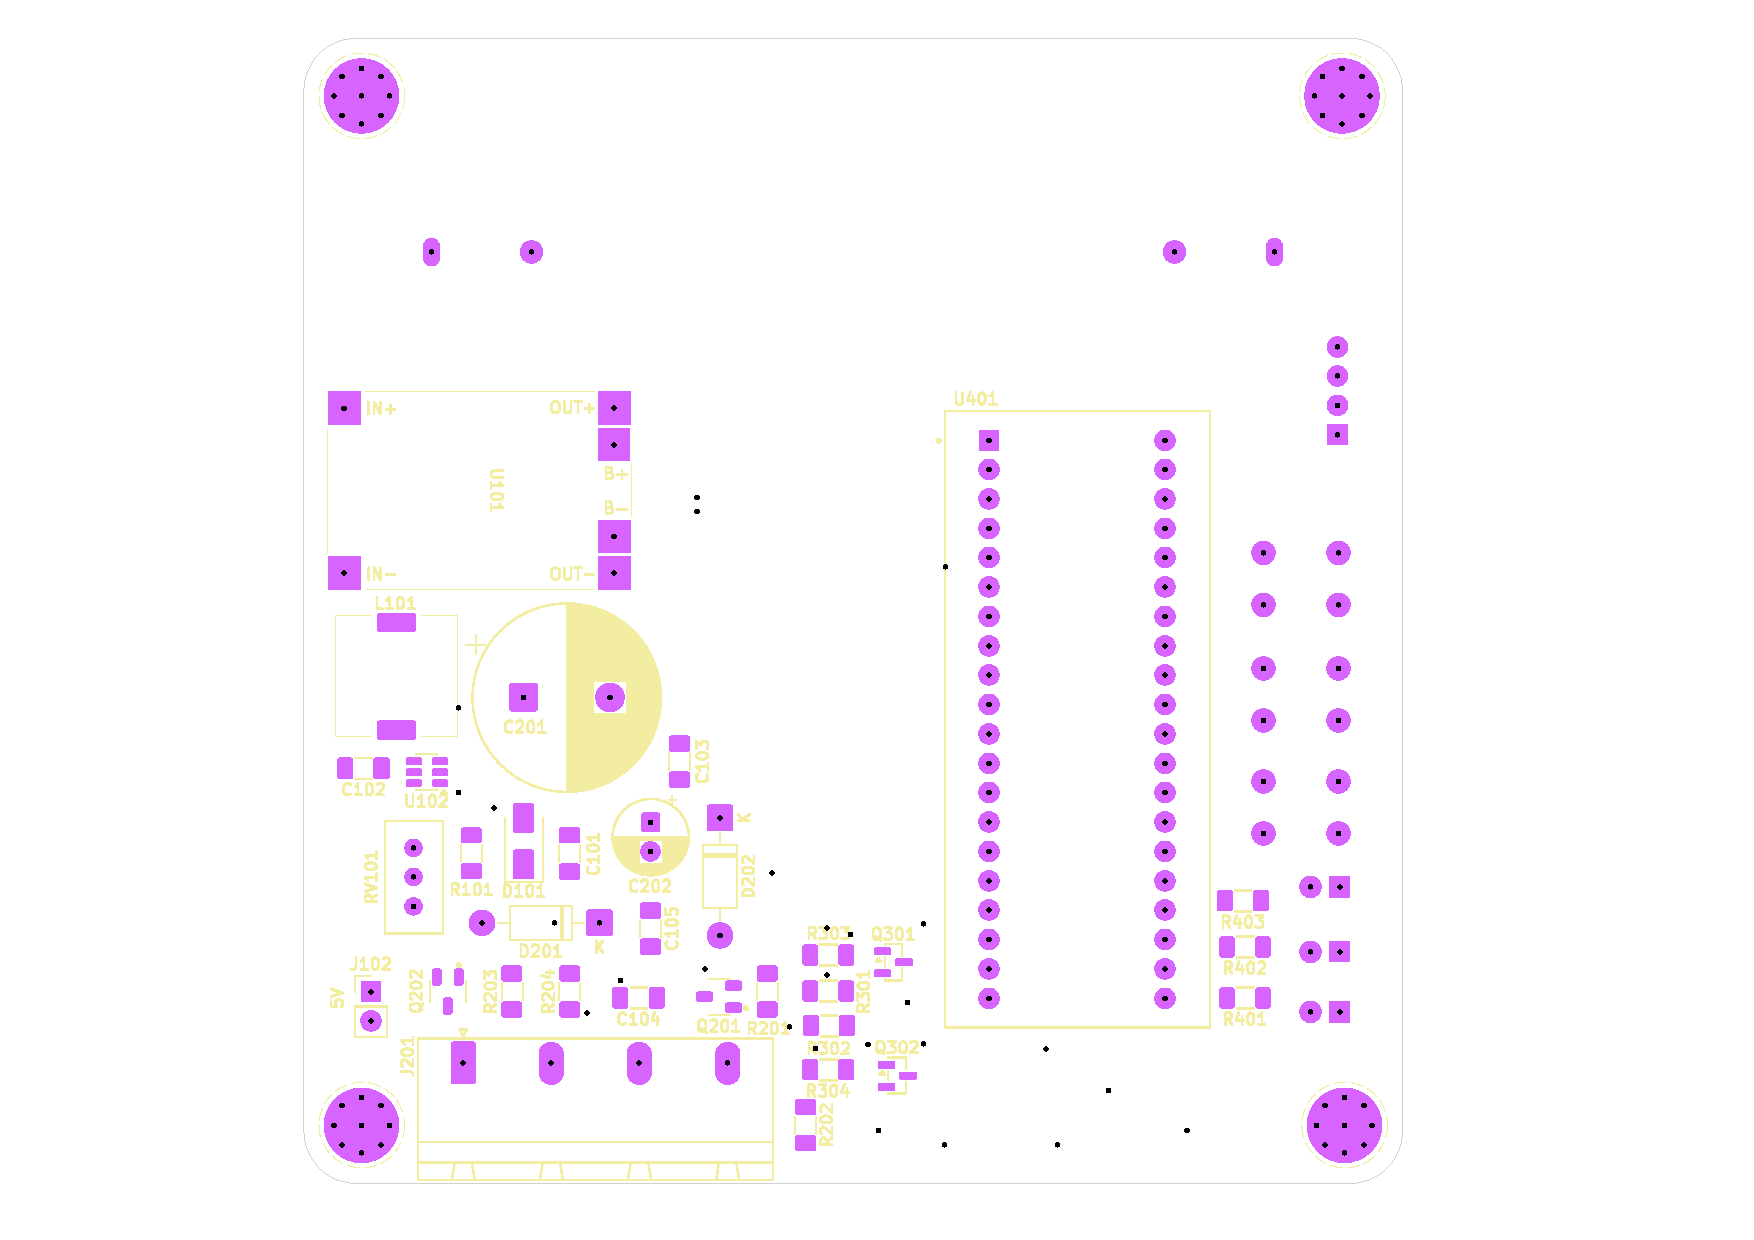
\includegraphics[width=0.95\textwidth]{images/schematic-print.pdf}
	\caption{Bản in schematic/board (trích từ dự án KiCad OscilloBP Monitor).}
	\label{fig:schematic-print}
\end{figure}

\section{Nhiệm vụ hiệu chỉnh phần cứng}
Để đọc mmHg chính xác từ ADC, cần hiệu chỉnh hai tham số trong firmware: \texttt{PRESSURE\_ADC\_OFFSET\_COUNTS} và \texttt{PRESSURE\_ADC\_SCALE\_MMHG\_PER\_COUNT} so với đồng hồ áp chuẩn hoặc nguồn áp đã biết. Đây là bước bắt buộc trước khi đánh giá lâm sàng.
